\documentclass[border=3pt]{standalone}
\usepackage{fontspec}
\usepackage{unicode-math}
\setmainfont{texgyretermes}[Extension=.otf, UprightFont=*-regular, BoldFont=*-bold,
  ItalicFont=*-italic, BoldItalicFont=*-bolditalic]
\setsansfont{texgyreheros}[Extension=.otf, UprightFont=*-regular, BoldFont=*-bold]
\setmathfont{texgyretermes-math.otf}
\newfontfamily\chessfont{Apple Symbols}
\usepackage{tikz}
\usepackage{pgfplots}
\pgfplotsset{compat=1.17}
\definecolor{light}{HTML}{EDEDED}
\definecolor{dark}{HTML}{7389B8}
\definecolor{edge}{HTML}{4A4A4A}
\definecolor{blue2}{HTML}{B9C6E0}
\begin{document}
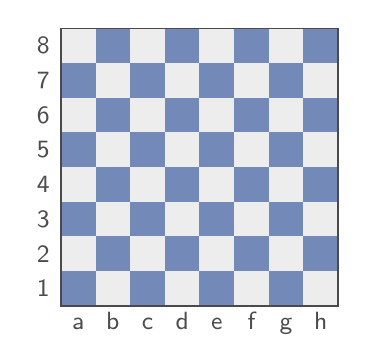
\begin{tikzpicture}[x=0.44cm,y=0.44cm]
\fill[dark] (0,0) rectangle (1,1);
\fill[light] (0,1) rectangle (1,2);
\fill[dark] (0,2) rectangle (1,3);
\fill[light] (0,3) rectangle (1,4);
\fill[dark] (0,4) rectangle (1,5);
\fill[light] (0,5) rectangle (1,6);
\fill[dark] (0,6) rectangle (1,7);
\fill[light] (0,7) rectangle (1,8);
\fill[light] (1,0) rectangle (2,1);
\fill[dark] (1,1) rectangle (2,2);
\fill[light] (1,2) rectangle (2,3);
\fill[dark] (1,3) rectangle (2,4);
\fill[light] (1,4) rectangle (2,5);
\fill[dark] (1,5) rectangle (2,6);
\fill[light] (1,6) rectangle (2,7);
\fill[dark] (1,7) rectangle (2,8);
\fill[dark] (2,0) rectangle (3,1);
\fill[light] (2,1) rectangle (3,2);
\fill[dark] (2,2) rectangle (3,3);
\fill[light] (2,3) rectangle (3,4);
\fill[dark] (2,4) rectangle (3,5);
\fill[light] (2,5) rectangle (3,6);
\fill[dark] (2,6) rectangle (3,7);
\fill[light] (2,7) rectangle (3,8);
\fill[light] (3,0) rectangle (4,1);
\fill[dark] (3,1) rectangle (4,2);
\fill[light] (3,2) rectangle (4,3);
\fill[dark] (3,3) rectangle (4,4);
\fill[light] (3,4) rectangle (4,5);
\fill[dark] (3,5) rectangle (4,6);
\fill[light] (3,6) rectangle (4,7);
\fill[dark] (3,7) rectangle (4,8);
\fill[dark] (4,0) rectangle (5,1);
\fill[light] (4,1) rectangle (5,2);
\fill[dark] (4,2) rectangle (5,3);
\fill[light] (4,3) rectangle (5,4);
\fill[dark] (4,4) rectangle (5,5);
\fill[light] (4,5) rectangle (5,6);
\fill[dark] (4,6) rectangle (5,7);
\fill[light] (4,7) rectangle (5,8);
\fill[light] (5,0) rectangle (6,1);
\fill[dark] (5,1) rectangle (6,2);
\fill[light] (5,2) rectangle (6,3);
\fill[dark] (5,3) rectangle (6,4);
\fill[light] (5,4) rectangle (6,5);
\fill[dark] (5,5) rectangle (6,6);
\fill[light] (5,6) rectangle (6,7);
\fill[dark] (5,7) rectangle (6,8);
\fill[dark] (6,0) rectangle (7,1);
\fill[light] (6,1) rectangle (7,2);
\fill[dark] (6,2) rectangle (7,3);
\fill[light] (6,3) rectangle (7,4);
\fill[dark] (6,4) rectangle (7,5);
\fill[light] (6,5) rectangle (7,6);
\fill[dark] (6,6) rectangle (7,7);
\fill[light] (6,7) rectangle (7,8);
\fill[light] (7,0) rectangle (8,1);
\fill[dark] (7,1) rectangle (8,2);
\fill[light] (7,2) rectangle (8,3);
\fill[dark] (7,3) rectangle (8,4);
\fill[light] (7,4) rectangle (8,5);
\fill[dark] (7,5) rectangle (8,6);
\fill[light] (7,6) rectangle (8,7);
\fill[dark] (7,7) rectangle (8,8);
\draw[edge, line width=0.6pt] (0,0) rectangle (8,8);
\node[anchor=east, text=black!70, font=\sffamily\fontsize{9}{9}\selectfont] at (-0.04,0.5) {1};
\node[anchor=east, text=black!70, font=\sffamily\fontsize{9}{9}\selectfont] at (-0.04,1.5) {2};
\node[anchor=east, text=black!70, font=\sffamily\fontsize{9}{9}\selectfont] at (-0.04,2.5) {3};
\node[anchor=east, text=black!70, font=\sffamily\fontsize{9}{9}\selectfont] at (-0.04,3.5) {4};
\node[anchor=east, text=black!70, font=\sffamily\fontsize{9}{9}\selectfont] at (-0.04,4.5) {5};
\node[anchor=east, text=black!70, font=\sffamily\fontsize{9}{9}\selectfont] at (-0.04,5.5) {6};
\node[anchor=east, text=black!70, font=\sffamily\fontsize{9}{9}\selectfont] at (-0.04,6.5) {7};
\node[anchor=east, text=black!70, font=\sffamily\fontsize{9}{9}\selectfont] at (-0.04,7.5) {8};
\node[anchor=north, text=black!70, text height=1.45ex, text depth=0.2ex, inner sep=1.5pt, font=\sffamily\fontsize{9}{9}\selectfont] at (0.5,-0.04) {a};
\node[anchor=north, text=black!70, text height=1.45ex, text depth=0.2ex, inner sep=1.5pt, font=\sffamily\fontsize{9}{9}\selectfont] at (1.5,-0.04) {b};
\node[anchor=north, text=black!70, text height=1.45ex, text depth=0.2ex, inner sep=1.5pt, font=\sffamily\fontsize{9}{9}\selectfont] at (2.5,-0.04) {c};
\node[anchor=north, text=black!70, text height=1.45ex, text depth=0.2ex, inner sep=1.5pt, font=\sffamily\fontsize{9}{9}\selectfont] at (3.5,-0.04) {d};
\node[anchor=north, text=black!70, text height=1.45ex, text depth=0.2ex, inner sep=1.5pt, font=\sffamily\fontsize{9}{9}\selectfont] at (4.5,-0.04) {e};
\node[anchor=north, text=black!70, text height=1.45ex, text depth=0.2ex, inner sep=1.5pt, font=\sffamily\fontsize{9}{9}\selectfont] at (5.5,-0.04) {f};
\node[anchor=north, text=black!70, text height=1.45ex, text depth=0.2ex, inner sep=1.5pt, font=\sffamily\fontsize{9}{9}\selectfont] at (6.5,-0.04) {g};
\node[anchor=north, text=black!70, text height=1.45ex, text depth=0.2ex, inner sep=1.5pt, font=\sffamily\fontsize{9}{9}\selectfont] at (7.5,-0.04) {h};
\node[text=white, inner sep=0] at (4.5,1.47) {\chessfont\fontsize{12.0}{12.0}\selectfont♟};
\node[text=black, inner sep=0] at (4.5,1.47) {\chessfont\fontsize{12.0}{12.0}\selectfont♙};
\node[text=black, inner sep=0] at (4.5,4.47) {\chessfont\fontsize{12.0}{12.0}\selectfont♟};
\end{tikzpicture}
\end{document}
